%Fig_LSTM_Main_Figure_3_Cells.tex
\begin{figure}[!ht]
\minipage{0.33\textwidth}
%\begin{tikzpicture}[scale=.9]

  % The grid
   %%\draw[step=0.5, gray!40, very thin] (-1.5,0) grid (8,4);

  % LSTM frame
  \def \yONE {0.5}
  \def \yTWO {3.3}
  \draw[rounded corners=12pt, very thick, gray,fill=LightGreen]  (-1.5, 0.5) rectangle (3.2, 3.3);

  \def \sigmoidWidth  {0.45}
  \def \sigmoidInDist {0.2}
  \def \sigmoidHeight  {0.3}
  \def \yB  {1.3}
  \def \yD  {2.75}
  \def \shift {0.3}
  % First Sigmoid
  \draw[thick,fill=yellow] (-1, \yB) rectangle (-1+ \sigmoidWidth, \yB + \sigmoidHeight) node[pos=0.5] {$\sigma$};

  \def \r {.15cm}
  % The Upper times operator % first time from left
  \draw[thick,fill=pink] (-.75, \yD) circle (\r) node {$\times$};

  % Second Sigmoid
  \def \xS {-.5 +\sigmoidInDist}
  \draw[thick,fill=yellow]  (\xS, \yB) rectangle (\xS +\sigmoidWidth, \yB + \sigmoidHeight) node[pos=0.5] {$\sigma$};

  % Square tanh
  \def \xSS {\xS +\sigmoidWidth + \sigmoidInDist}
  \draw[thick,fill=yellow]  (\xSS, \yB) 
  rectangle 
  (\xSS +\sigmoidWidth, \yB +\sigmoidHeight)
  node[pos=0.5] {\scriptsize \textit{tanh}};

  % Third Sigoid
  \def \xSSS {\xSS +\sigmoidWidth +0.13 +\sigmoidInDist}
  \draw[thick,fill=yellow]  (\xSSS, \yB) rectangle (\xSSS +\sigmoidWidth, \yB +\sigmoidHeight)
  node[pos=0.5] { $\sigma$};

  % Second times operator and add operator
  \def \xTimesB {.5}
  \def \yC      {2}

  \draw[thick,fill=pink] (\xTimesB, \yC) circle (\r) node {$\times$};
  
  %%%%% **first line sectond operator +
  \draw[thick,fill=pink] (\xTimesB, \yD) circle (\r) node {$+$};

  % Third times operator 
  \draw[thick,fill=pink] (\xTimesB +1.3 +\shift, \yC) circle (\r) node {$\times$};
  
  %second tanh 
  \draw[thick,fill=yellow] (\xTimesB +1.3 +\shift, \yC +.4)  
  ellipse (.35cm and .14cm) 
  node {\scriptsize \textit{tanh}};


  % LINES %%% Upper line from c_{t -1} till C_t
  %\draw[arrows=-latex, line width=1.5pt,gray]  (-2.15, \yD) -- (-1.5, \yD) node[left, xshift=-.6cm, yshift=0.2cm] {$C_{t-1}$};
  \draw[line width=1.5pt,gray]  (-1.5, \yD) -- (-.9, \yD);
  \draw[line width=1.5pt,gray]  (-.6, \yD) -- (.35, \yD);
  \draw[line width=1.5pt,gray]  (.68, \yD) -- (3.2, \yD);
  \draw[arrows=-latex, line width=2.5pt]  (3.2, \yD) -- (4.3, \yD);% node[right, xshift=0.0cm, yshift=0.05cm] {$C_t$};


  %%%%first line from left from sigmoid ft till times input from C_{t-1}
  \draw[arrows=-latex, line width=1.5pt,gray]  (-.75, \yB +\sigmoidHeight) -- (-.75, 2.6)
  node[left, yshift=-0.5cm] {$f_t$};

  % Level B LINES
  \def \levelB {1}
  %input h_{t-1} line
  
   %\draw[arrows=-latex, line width=1.5pt,gray]  (-2.15, \levelB) -- (-1.5, \levelB)    node[left, xshift=-.6cm, yshift=0.2cm] {$h_{t-1}$};

%level B line base between input h_{t-1} and first sigmoid
  \draw[line width=1.5pt,gray] (-1.5, \levelB) -- (.75, \levelB);
  
  %level B line base between  first sigmoid and tanh%more
   \draw[line width=1.5pt,gray] (.5, \levelB) --  (1.2, \levelB);
  
    \def \xOfThirdSigmoid {\xSSS + \sigmoidWidth/2}
  %second line last angle connected to sigmoid 
  \draw[line width=1.5pt,gray] (1.2, \levelB) to[out=0,in=270] (\xOfThirdSigmoid, \yB);
  
  %level B line base between  tanh and tanh angle--------
  \draw[line width=1.5pt,gray] (2.25, \levelB) -- (2.56, \levelB);



  % Third Sigmoid up line
  % END (\xTimesB +1.3 - 0.19 , \yC)
  \draw[line width=1.5pt,gray] (\xOfThirdSigmoid, \yB + \sigmoidHeight) 
  --
  (\xOfThirdSigmoid, \yB + \sigmoidHeight + 0.17) ;

  \draw[arrows=-latex, line width=1.5pt,gray] (\xOfThirdSigmoid, \yB + \sigmoidHeight+0.17) 
  to[out=90, in=180] 
  (\xTimesB +1.3 -0.14 +\shift , \yC) 
  node [left, yshift=0.2cm, xshift=-0.2cm] {$o_t$};

  % tanh line from line B to third tirangle tanh
  \draw [line width=1.5pt,gray] (\xTimesB, \levelB)   --   (\xTimesB, \yB);

%line between first tanh from left and x %%%%
  \draw [line width=1.5pt,gray] (\xTimesB, \yB + \sigmoidHeight)
  --
  (\xTimesB, \yB + \sigmoidHeight +0.24)
  node [left, yshift=-0.1cm, xshift=-0.1cm] {$\tilde{C_t}$};

%line between x and + upper first tanh from left
  \draw [arrows=-latex, line width=1.5pt,gray] (\xTimesB, 2.15)   --   (\xTimesB, 2.6);

%line between level B and first sigmoid
  \draw[line width=1.5pt,gray] (-.75, \levelB)  --  (-.75, \yB);
  
  % line between level B and second sigmoid
  \draw[line width=1.5pt,gray] (\xS +\sigmoidWidth/2, \levelB)
  --
  (\xS +\sigmoidWidth/2, \yB);

% line angle between sgima and x midlle line
  \draw[line width=1.5pt,gray] (\xS +\sigmoidWidth/2, \yB +\sigmoidHeight)
  -- 
  (\xS +\sigmoidWidth/2, \yB +\sigmoidHeight + 0.17);

  %% angle between sgima and x midlle line i_t
  \draw[arrows=-latex, line width=1.5pt,gray] (\xS +\sigmoidWidth/2, \yB + \sigmoidHeight+0.17) 
  to[out=90, in=180] 
  (\xTimesB-0.14, \yC)
  node [left, yshift=0.2cm, xshift=-0.2cm] {$i_t$};

  \def \bigR {0.25cm}
  \def \bigRTWO {0.4cm}
  \def \C    {1}
  \def \xBigCicleONE {2}
  \def \xBigCicleTWO {5.5 + 0.25}
  \draw[thick,fill=LightBlue] (\xBigCicleONE-3, \yONE -.15- \C) circle (\bigRTWO) node {$x_{t-1}$};
  \draw[thick,fill=LightPurple] (\xBigCicleTWO-3, \yTWO +.2+ \C) circle (\bigRTWO) node {$h_{t-1}$};

  
  % LINE Circle ONE from xt to line B
  \draw[line width=1.5pt,gray] (-3+\xBigCicleONE, \yONE -\C +0.25) 
  --
  (\xBigCicleONE-3, \yONE -\C +0.25 + 1.1);

%% angle from the x_t to sigma ifrst angle from the left down
  \draw[line width=1.5pt,gray] (\xBigCicleONE-3, \yONE -\C +0.25 + 1.1)
  to[out=90, in=180]
  (-.75, 1);

  % LINE third \times betweem line B and times circle 
  \draw[line width=1.5pt,gray] (\xTimesB +1.3 +\shift, 1.1)
  --
  (\xTimesB +1.3 +\shift, \yC - 0.15);


%level A line
  \draw[line width=1.5pt,gray] (2.56, \levelB)
  --
  (3.2,\levelB);

\draw[arrows=-latex, line width=2.5pt] (3.2, \levelB) 
  --
  (4.3, \levelB);%  node[right, xshift=0.0cm, yshift=0.05cm,] {$h_t$};

  
%%% second line last angle connect the input with h_t output
  \draw[line width=1.5pt,gray] ( 2.1, 1.12)
  to[out=270, in=180]
  (2.3, 1);


%%% line between times and tanh (last tanh h on the right alone)
  \draw[line width=1.5pt,gray] (\xTimesB +1.3 +\shift, 2.14)
  --
  (\xTimesB +1.3 +\shift, 2.26);

%%%%% Line between tanh and Line level A 
  \draw[line width=1.5pt,gray] (\xTimesB +1.3 +\shift, \yD)
  --
  (\xTimesB +1.3 +\shift, 2.54);

%%%%% first horizontal line from the right angle connected to the line which connect to output ht
  \draw[line width=1.5pt,gray] (\xBigCicleTWO-3, \levelB +0.2)
  --
  (\xBigCicleTWO-3, \yTWO);

%%%%% first horizontal line from the right angle connected to output ht
  \draw[line width=1.5pt,gray] (\xBigCicleTWO - 3.2, \levelB)
  to[out=0, in=270]
  (\xBigCicleTWO-3, \levelB +0.25);

%%%%% first horizontal line from the right angle connected to output ht

  \draw[arrows=-latex, line width=1.5pt,gray]
  (\xBigCicleTWO-3, \yD +.55)
  --
  (\xBigCicleTWO-3, 4.1);
  
\end{tikzpicture}

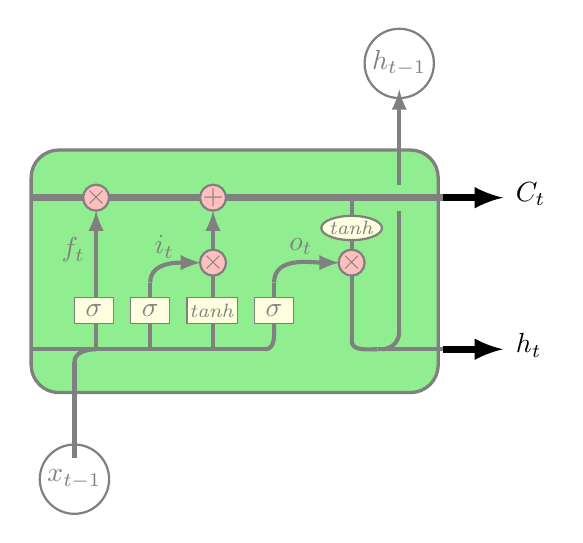
\begin{tikzpicture}[scale=1.1]

  % The grid
  % \draw[step=0.5, gray!40, very thin] (0,0) grid (8,4);

  % LSTM frame
  \def \yONE {0.5}
  \def \yTWO {3.3}
  \draw[rounded corners=10pt, very thick, gray,fill=LightGreen]  (1.5, 0.5) rectangle (6.2, 3.3);

  \def \sigmoidWidth  {0.45}
  \def \sigmoidInDist {0.2}
  \def \sigmoidHeight  {0.3}
  \def \yB  {1.3}
  \def \yD  {2.75}
  \def \shift {0.3}
  % First Sigmoid
  \draw[gray,fill=LightYellow] (2, \yB) rectangle (2+ \sigmoidWidth, \yB + \sigmoidHeight) node[pos=0.5] {$\sigma$};

  \def \r {.15cm}
  % The Upper times operator % first time from left
  \draw[thick, gray,fill=pink] (2.25, \yD) circle (\r) node {$\times$};

  % Second Sigmoid
  \def \xS {2.45 +\sigmoidInDist}
  \draw[gray,fill=LightYellow]  (\xS, \yB) rectangle (\xS +\sigmoidWidth, \yB + \sigmoidHeight) node[pos=0.5] {$\sigma$};

  % Square tanh
  \def \xSS {\xS +\sigmoidWidth + \sigmoidInDist}
  \draw[gray,fill=LightYellow]  (\xSS, \yB) 
  rectangle 
  (\xSS +\sigmoidWidth +0.13, \yB +\sigmoidHeight)
  node[pos=0.5] {\scriptsize \textit{tanh}};

  % Third Sigoid
  \def \xSSS {\xSS +\sigmoidWidth +0.13 +\sigmoidInDist}
  \draw[gray,fill=LightYellow]  (\xSSS, \yB) rectangle (\xSSS +\sigmoidWidth, \yB +\sigmoidHeight)
  node[pos=0.5] { $\sigma$};

  % Second times operator and add operator
  \def \xTimesB {3.6}
  \def \yC      {2}

  \draw[thick,gray,fill=pink] (\xTimesB, \yC) circle (\r) node {$\times$};
  %%%%% first line sectond operator +
  \draw[thick, gray,fill=pink] (\xTimesB, \yD) circle (\r) node {$+$};

  % Third times operator and its tanh
  \draw[thick,gray,fill=pink] (\xTimesB +1.3 +\shift, \yC) circle (\r) node {$\times$};
  \draw[thick,gray,fill=LightYellow] (\xTimesB +1.3 +\shift, \yC +.4)  
  ellipse (.35cm and .14cm) 
  node {\scriptsize \textit{tanh}};


  % LINES %%% Upper line from c_{t -1} till C_t
  %\draw[arrows=-latex, line width=2.5pt]  (0.85, \yD) -- (1.5, \yD) node[left, xshift=-.6cm, yshift=0.2cm] {$C_{t-1}$};
  \draw[line width=2.5pt, gray]  (1.5, \yD) -- (2.1, \yD);
  \draw[line width=2.5pt, gray]  (2.4, \yD) -- (3.46, \yD);
  \draw[line width=2.5pt,gray]  (3.75, \yD) -- (6.25 +0.2, \yD);

  \draw[arrows=-latex, line width=2.5pt]  (6.25, \yD) -- (6.75 +0.2, \yD)
  node[right, xshift=0.0cm, yshift=0.05cm] {$C_t$};

  %%%%first line from left from sigmoid ft till times input from C_{t-1}
  \draw[arrows=-latex, line width=1.5pt,gray]  (2.25, \yB +\sigmoidHeight) -- (2.25, 2.6)
  node[left, yshift=-0.5cm] {$f_t$};

  % Level B LINES
  \def \levelB {1}
  %\draw[arrows=-latex, line width=1.5pt,gray] (0.85, \levelB) -- (1.5, \levelB) node[left, xshift=-.6cm, yshift=0.2cm] {$h_{t-1}$};

  \draw[line width=1.5pt,gray] (1.5, \levelB) 
  --
  (4.2, \levelB);

  \def \xOfThirdSigmoid {\xSSS + \sigmoidWidth/2}
  %second line last angle connected to sigmoid 
  \draw[line width=1.5pt,gray] (4.2, \levelB) to[out=0,in=270] (\xOfThirdSigmoid, \yB);

  % Third Sigmoid up line
  % END (\xTimesB +1.3 - 0.19 , \yC)
  \draw[line width=1.5pt,gray] (\xOfThirdSigmoid, \yB + \sigmoidHeight) 
  --
  (\xOfThirdSigmoid, \yB + \sigmoidHeight + 0.17) ;

  \draw[arrows=-latex, line width=1.5pt,gray] (\xOfThirdSigmoid, \yB + \sigmoidHeight+0.17) 
  to[out=90, in=180] 
  (\xTimesB +1.3 -0.14 +\shift , \yC) 
  node [left, yshift=0.2cm, xshift=-0.2cm] {$o_t$};

  % tanh line
  \draw [line width=1.5pt,gray] (\xTimesB, \levelB)
  --
  (\xTimesB, \yB);

  \draw [line width=1.5pt,gray] (\xTimesB, \yB + \sigmoidHeight)
  --
  (\xTimesB, \yB + \sigmoidHeight +0.24);

  \draw [arrows=-latex, line width=1.5pt,gray] (\xTimesB, 2.15)
  --
  (\xTimesB, 2.6);

  \draw[line width=1.5pt,gray] (2.25, \levelB)
  --
  (2.25, \yB);
  
  \draw[line width=1.5pt,gray] (\xS +\sigmoidWidth/2, \levelB)
  --
  (\xS +\sigmoidWidth/2, \yB);

  \draw[line width=1.5pt,gray] (\xS +\sigmoidWidth/2, \yB +\sigmoidHeight)
  -- 
  (\xS +\sigmoidWidth/2, \yB +\sigmoidHeight + 0.17);

  \draw[arrows=-latex, line width=1.5pt,gray] (\xS +\sigmoidWidth/2, \yB + \sigmoidHeight+0.17) 
  to[out=90, in=180] 
  (\xTimesB-0.14, \yC)
  node [left, yshift=0.2cm, xshift=-0.2cm] {$i_t$};

  \def \bigR {0.25cm}
  \def \bigRTWO {0.4cm}
  \def \C    {1}
  \def \xBigCicleONE {2}
  \def \xBigCicleTWO {5.5 + 0.25}
  \draw[thick,gray] (\xBigCicleONE, \yONE - \C) circle (\bigRTWO) node {$x_{t-1}$};
  \draw[thick,gray] (\xBigCicleTWO, \yTWO + \C) circle (\bigRTWO) node {$h_{t-1}$};

  % LINE Circle ONE
  \draw[line width=1.5pt,gray] (\xBigCicleONE, \yONE -\C +0.25) 
  --
  (\xBigCicleONE, \yONE -\C +0.25 + 1.1);

  \draw[line width=1.5pt,gray] (\xBigCicleONE, \yONE -\C +0.25 + 1.1)
  to[out=90, in=180]
  (2.25, 1);

  % LINE third \times
  \draw[line width=1.5pt,gray] (\xTimesB +1.3 +\shift, 1.1)
  --
  (\xTimesB +1.3 +\shift, \yC - 0.15);

  \draw[line width=1.5pt,gray] (5.5, 1) 
  --
  (6.25 +0.2, 1);
  
  \draw[arrows=-latex,line width=2.5pt] (6.25, 1) 
  --
  (6.75 +0.2, 1)
  node[right, xshift=0.0cm, yshift=0.05cm,] {$h_t$};

%%% second line last angle connect the input with h_t output
  \draw[line width=1.5pt,gray] (\xTimesB +1.3 +\shift, 1.1)
  to[out=270, in=180]
  (5.5, 1);


  \draw[line width=1.5pt,gray] (\xTimesB +1.3 +\shift, 2.14)
  --
  (\xTimesB +1.3 +\shift, 2.26);


  \draw[line width=1.5pt,gray] (\xTimesB +1.3 +\shift, \yD)
  --
  (\xTimesB +1.3 +\shift, 2.54);


  \draw[line width=1.5pt,gray] (\xBigCicleTWO, \levelB +0.2)
  --
  (\xBigCicleTWO, 2.6);

%%%%% first horizontal line from the right angle connected to output ht
  \draw[line width=1.5pt,gray] (\xBigCicleTWO - 0.2, \levelB)
  to[out=0, in=270]
  (\xBigCicleTWO, \levelB +0.2);


  \draw[arrows=-latex, line width=1.5pt,gray]
  (\xBigCicleTWO, \yD +0.15)
  --
  (\xBigCicleTWO, 4);

\end{tikzpicture}



\endminipage\hfill
\minipage{0.33\textwidth}
% \begin{tikzpicture}%[scale=.9]

  % The grid
   %%\draw[step=0.5, gray!40, very thin] (-1.5,0) grid (8,4);

  % LSTM frame
  \def \yONE {0.5}
  \def \yTWO {3.3}
  \draw[rounded corners=12pt, very thick, gray,fill=LightGreen]  (-1.5, 0.5) rectangle (3.2, 3.3);

  \def \sigmoidWidth  {0.45}
  \def \sigmoidInDist {0.2}
  \def \sigmoidHeight  {0.3}
  \def \yB  {1.3}
  \def \yD  {2.75}
  \def \shift {0.3}
  % First Sigmoid
  \draw[thick,fill=yellow] (-1, \yB) rectangle (-1+ \sigmoidWidth, \yB + \sigmoidHeight) node[pos=0.5] {$\sigma$};

  \def \r {.15cm}
  % The Upper times operator % first time from left
  \draw[thick,fill=pink] (-.75, \yD) circle (\r) node {$\times$};

  % Second Sigmoid
  \def \xS {-.5 +\sigmoidInDist}
  \draw[thick,fill=yellow]  (\xS, \yB) rectangle (\xS +\sigmoidWidth, \yB + \sigmoidHeight) node[pos=0.5] {$\sigma$};

  % Square tanh
  \def \xSS {\xS +\sigmoidWidth + \sigmoidInDist}
  \draw[thick,fill=yellow]  (\xSS, \yB) 
  rectangle 
  (\xSS +\sigmoidWidth, \yB +\sigmoidHeight)
  node[pos=0.5] {\scriptsize \textit{tanh}};

  % Third Sigoid
  \def \xSSS {\xSS +\sigmoidWidth +0.13 +\sigmoidInDist}
  \draw[thick,fill=yellow]  (\xSSS, \yB) rectangle (\xSSS +\sigmoidWidth, \yB +\sigmoidHeight)
  node[pos=0.5] { $\sigma$};

  % Second times operator and add operator
  \def \xTimesB {.5}
  \def \yC      {2}

  \draw[thick,fill=pink] (\xTimesB, \yC) circle (\r) node {$\times$};
  
  %%%%% **first line sectond operator +
  \draw[thick,fill=pink] (\xTimesB, \yD) circle (\r) node {$+$};

  % Third times operator 
  \draw[thick,fill=pink] (\xTimesB +1.3 +\shift, \yC) circle (\r) node {$\times$};
  
  %second tanh 
  \draw[thick,fill=yellow] (\xTimesB +1.3 +\shift, \yC +.4)  
  ellipse (.35cm and .14cm) 
  node {\scriptsize \textit{tanh}};


  % LINES %%% Upper line from c_{t -1} till C_t
  %\draw[arrows=-latex, line width=2.5pt]  (-2.15, \yD) -- (-1.5, \yD) node[left, xshift=-.6cm, yshift=0.2cm] {$C_{t-1}$};
  \draw[line width=2.5pt]  (-1.5, \yD) -- (-.9, \yD);
  \draw[line width=2.5pt]  (-.6, \yD) -- (.35, \yD);
  \draw[arrows=-latex, line width=2.5pt]  (.65, \yD) -- (4.3, \yD) node[right, xshift=0.0cm, yshift=0.05cm] {$C_t$};


  %%%%first line from left from sigmoid ft till times input from C_{t-1}
  \draw[arrows=-latex, line width=2.5pt]  (-.75, \yB +\sigmoidHeight) -- (-.75, 2.6)
  node[left, yshift=-0.5cm] {$f_t$};

  % Level B LINES
  \def \levelB {1}
  %input h_{t-1} line
  
   %\draw[arrows=-latex, line width=2.5pt]  (-2.15, \levelB) -- (-1.5, \levelB)    node[left, xshift=-.6cm, yshift=0.2cm] {$h_{t-1}$};

%level B line base between input h_{t-1} and first sigmoid
  \draw[line width=2.5pt] (-1.5, \levelB) -- (.75, \levelB);
  
  %level B line base between  first sigmoid and tanh%more
   \draw[line width=2.5pt] (.5, \levelB) --  (1.2, \levelB);
  
    \def \xOfThirdSigmoid {\xSSS + \sigmoidWidth/2}
  %second line last angle connected to sigmoid 
  \draw[line width=2.5pt] (1.2, \levelB) to[out=0,in=270] (\xOfThirdSigmoid, \yB);
  
  %level B line base between  tanh and tanh angle--------
  \draw[line width=2.5pt] (2.25, \levelB) -- (2.56, \levelB);



  % Third Sigmoid up line
  % END (\xTimesB +1.3 - 0.19 , \yC)
  \draw[line width=2.5pt] (\xOfThirdSigmoid, \yB + \sigmoidHeight) 
  --
  (\xOfThirdSigmoid, \yB + \sigmoidHeight + 0.17) ;

  \draw[arrows=-latex, line width=2.5pt] (\xOfThirdSigmoid, \yB + \sigmoidHeight+0.17) 
  to[out=90, in=180] 
  (\xTimesB +1.3 -0.14 +\shift , \yC) 
  node [left, yshift=0.2cm, xshift=-0.2cm] {$o_t$};

  % tanh line from line B to third tirangle tanh
  \draw [line width=2.5pt] (\xTimesB, \levelB)   --   (\xTimesB, \yB);

%line between first tanh from left and x %%%%
  \draw [line width=2.5pt] (\xTimesB, \yB + \sigmoidHeight)
  --
  (\xTimesB, \yB + \sigmoidHeight +0.24)
  node [left, yshift=-0.1cm, xshift=-0.1cm] {$\tilde{C_t}$};

%line between x and + upper first tanh from left
  \draw [arrows=-latex, line width=2.5pt] (\xTimesB, 2.15)   --   (\xTimesB, 2.6);

%line between level B and first sigmoid
  \draw[line width=2.5pt] (-.75, \levelB)  --  (-.75, \yB);
  
  % line between level B and second sigmoid
  \draw[line width=2.5pt] (\xS +\sigmoidWidth/2, \levelB)
  --
  (\xS +\sigmoidWidth/2, \yB);

% line angle between sgima and x midlle line
  \draw[line width=2.5pt] (\xS +\sigmoidWidth/2, \yB +\sigmoidHeight)
  -- 
  (\xS +\sigmoidWidth/2, \yB +\sigmoidHeight + 0.17);

  %% angle between sgima and x midlle line i_t
  \draw[arrows=-latex, line width=2.5pt] (\xS +\sigmoidWidth/2, \yB + \sigmoidHeight+0.17) 
  to[out=90, in=180] 
  (\xTimesB-0.14, \yC)
  node [left, yshift=0.2cm, xshift=-0.2cm] {$i_t$};

  \def \bigR {0.25cm}
  \def \bigRTWO {0.4cm}
  \def \C    {1}
  \def \xBigCicleONE {2}
  \def \xBigCicleTWO {5.5 + 0.25}
  \draw[thick,fill=LightBlue] (\xBigCicleONE-3, \yONE -.15 - \C) circle (\bigRTWO) node {$x_t$};
  \draw[thick,fill=LightPurple] (\xBigCicleTWO-3, \yTWO +.2+ \C) circle (\bigRTWO) node {$h_t$};
  %\draw[thick,gray] (\xBigCicleONE-3, \yONE -.15- \C) circle (\bigRTWO) node {$x_{t-1}$};
  %\draw[thick,gray] (\xBigCicleTWO-3, \yTWO +.2+ \C) circle (\bigRTWO) node {$h_{t-1}$};

  % LINE Circle ONE from xt to line B
  \draw[line width=2.5pt] (-3+\xBigCicleONE, \yONE -\C +0.25) 
  --
  (\xBigCicleONE-3, \yONE -\C +0.25 + 1.1);

%% angle from the x_t to sigma ifrst angle from the left down
  \draw[line width=2.5pt] (\xBigCicleONE-3, \yONE -\C +0.25 + 1.1)
  to[out=90, in=180]
  (-.75, 1);

  % LINE third \times betweem line B and times circle 
  \draw[line width=2.5pt] (\xTimesB +1.3 +\shift, 1.1)
  --
  (\xTimesB +1.3 +\shift, \yC - 0.15);

  
  \draw[arrows=-latex, line width=2.5pt] (2.56, \levelB) 
  --
  (4.3, \levelB)
  node[right, xshift=0.0cm, yshift=0.05cm,] {$h_t$};

%%% second line last angle connect the input with h_t output
  \draw[line width=2.5pt] ( 2.1, 1.12)
  to[out=270, in=180]
  (2.3, 1);


%%% line between times and tanh (last tanh h on the right alone)
  \draw[line width=2.5pt] (\xTimesB +1.3 +\shift, 2.14)
  --
  (\xTimesB +1.3 +\shift, 2.26);

%%%%% Line between tanh and Line level A 
  \draw[line width=2.5pt] (\xTimesB +1.3 +\shift, \yD)
  --
  (\xTimesB +1.3 +\shift, 2.54);

%%%%% first horizontal line from the right angle connected to the line which connect to output ht
  \draw[line width=2.5pt] (\xBigCicleTWO-3, \levelB +0.2)
  --
  (\xBigCicleTWO-3, \yTWO);

%%%%% first horizontal line from the right angle connected to output ht
  \draw[line width=2.5pt] (\xBigCicleTWO - 3.2, \levelB)
  to[out=0, in=270]
  (\xBigCicleTWO-3, \levelB +0.25);

%%%%% first horizontal line from the right angle connected to output ht

  \draw[arrows=-latex, line width=2.5pt]
  (\xBigCicleTWO-3, \yD +.55)
  --
  (\xBigCicleTWO-3, 4.1);
  
\end{tikzpicture}


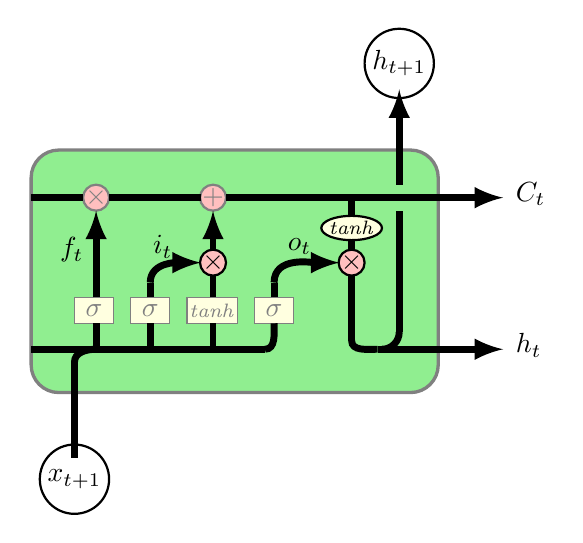
\begin{tikzpicture}[scale=1.1]

  % The grid
  % \draw[step=0.5, gray!40, very thin] (0,0) grid (8,4);

  % LSTM frame
  \def \yONE {0.5}
  \def \yTWO {3.3}
  \draw[rounded corners=10pt, very thick, gray,fill=LightGreen]  (1.5, 0.5) rectangle (6.2, 3.3);

  \def \sigmoidWidth  {0.45}
  \def \sigmoidInDist {0.2}
  \def \sigmoidHeight  {0.3}
  \def \yB  {1.3}
  \def \yD  {2.75}
  \def \shift {0.3}
  % First Sigmoid
  \draw[gray,fill=LightYellow] (2, \yB) rectangle (2+ \sigmoidWidth, \yB + \sigmoidHeight) node[pos=0.5] {$\sigma$};

  \def \r {.15cm}
  % The Upper times operator % first time from left
  \draw[thick, gray,fill=pink] (2.25, \yD) circle (\r) node {$\times$};

  % Second Sigmoid
  \def \xS {2.45 +\sigmoidInDist}
  \draw[gray,fill=LightYellow]  (\xS, \yB) rectangle (\xS +\sigmoidWidth, \yB + \sigmoidHeight) node[pos=0.5] {$\sigma$};

  % Square tanh
  \def \xSS {\xS +\sigmoidWidth + \sigmoidInDist}
  \draw[gray,fill=LightYellow]  (\xSS, \yB) 
  rectangle 
  (\xSS +\sigmoidWidth +0.13, \yB +\sigmoidHeight)
  node[pos=0.5] {\scriptsize \textit{tanh}};

  % Third Sigoid
  \def \xSSS {\xSS +\sigmoidWidth +0.13 +\sigmoidInDist}
  \draw[gray,fill=LightYellow]  (\xSSS, \yB) rectangle (\xSSS +\sigmoidWidth, \yB +\sigmoidHeight)
  node[pos=0.5] { $\sigma$};

  % Second times operator and add operator
  \def \xTimesB {3.6}
  \def \yC      {2}

  \draw[thick,fill=pink] (\xTimesB, \yC) circle (\r) node {$\times$};
  %%%%% first line sectond operator +
  \draw[thick, gray,fill=pink] (\xTimesB, \yD) circle (\r) node {$+$};

  % Third times operator and its tanh
  \draw[thick,fill=pink] (\xTimesB +1.3 +\shift, \yC) circle (\r) node {$\times$};
  \draw[thick,fill=LightYellow] (\xTimesB +1.3 +\shift, \yC +.4)  
  ellipse (.35cm and .14cm) 
  node {\scriptsize \textit{tanh}};


  % LINES %%% Upper line from c_{t -1} till C_t
  %\draw[arrows=-latex, line width=2.5pt]  (0.85, \yD) -- (1.5, \yD) node[left, xshift=-.6cm, yshift=0.2cm] {$C_{t-1}$};
  \draw[line width=2.5pt]  (1.5, \yD) -- (2.1, \yD);
  \draw[line width=2.5pt]  (2.4, \yD) -- (3.46, \yD);
  \draw[line width=2.5pt]  (3.75, \yD) -- (6.25 +0.2, \yD);

  \draw[arrows=-latex, line width=2.5pt]  (6.25, \yD) -- (6.75 +0.2, \yD)
  node[right, xshift=0.0cm, yshift=0.05cm] {$C_t$};

  %%%%first line from left from sigmoid ft till times input from C_{t-1}
  \draw[arrows=-latex, line width=2.5pt]  (2.25, \yB +\sigmoidHeight) -- (2.25, 2.6)
  node[left, yshift=-0.5cm] {$f_t$};

  % Level B LINES
  \def \levelB {1}
  %\draw[arrows=-latex, line width=2.5pt] (0.85, \levelB) -- (1.5, \levelB) node[left, xshift=-.6cm, yshift=0.2cm] {$h_{t-1}$};

  \draw[line width=2.5pt] (1.5, \levelB) 
  --
  (4.2, \levelB);

  \def \xOfThirdSigmoid {\xSSS + \sigmoidWidth/2}
  %second line last angle connected to sigmoid 
  \draw[line width=2.5pt] (4.2, \levelB) to[out=0,in=270] (\xOfThirdSigmoid, \yB);

  % Third Sigmoid up line
  % END (\xTimesB +1.3 - 0.19 , \yC)
  \draw[line width=2.5pt] (\xOfThirdSigmoid, \yB + \sigmoidHeight) 
  --
  (\xOfThirdSigmoid, \yB + \sigmoidHeight + 0.17) ;

  \draw[arrows=-latex, line width=2.5pt] (\xOfThirdSigmoid, \yB + \sigmoidHeight+0.17) 
  to[out=90, in=180] 
  (\xTimesB +1.3 -0.14 +\shift , \yC) 
  node [left, yshift=0.2cm, xshift=-0.2cm] {$o_t$};

  % tanh line
  \draw [line width=2.5pt] (\xTimesB, \levelB)
  --
  (\xTimesB, \yB);

  \draw [line width=2.5pt] (\xTimesB, \yB + \sigmoidHeight)
  --
  (\xTimesB, \yB + \sigmoidHeight +0.24);

  \draw [arrows=-latex, line width=2.5pt] (\xTimesB, 2.15)
  --
  (\xTimesB, 2.6);

  \draw[line width=2.5pt] (2.25, \levelB)
  --
  (2.25, \yB);
  
  \draw[line width=2.5pt] (\xS +\sigmoidWidth/2, \levelB)
  --
  (\xS +\sigmoidWidth/2, \yB);

  \draw[line width=2.5pt] (\xS +\sigmoidWidth/2, \yB +\sigmoidHeight)
  -- 
  (\xS +\sigmoidWidth/2, \yB +\sigmoidHeight + 0.17);

  \draw[arrows=-latex, line width=2.5pt] (\xS +\sigmoidWidth/2, \yB + \sigmoidHeight+0.17) 
  to[out=90, in=180] 
  (\xTimesB-0.14, \yC)
  node [left, yshift=0.2cm, xshift=-0.2cm] {$i_t$};

  \def \bigR {0.25cm}
  \def \bigRTWO {0.4cm}
  \def \C    {1}
  \def \xBigCicleONE {2}
  \def \xBigCicleTWO {5.5 + 0.25}
  \draw[thick] (\xBigCicleONE, \yONE - \C) circle (\bigRTWO) node {$x_{t+1}$};
  \draw[thick] (\xBigCicleTWO, \yTWO + \C) circle (\bigRTWO) node {$h_{t+1}$};

  % LINE Circle ONE
  \draw[line width=2.5pt] (\xBigCicleONE, \yONE -\C +0.25) 
  --
  (\xBigCicleONE, \yONE -\C +0.25 + 1.1);

  \draw[line width=2.5pt] (\xBigCicleONE, \yONE -\C +0.25 + 1.1)
  to[out=90, in=180]
  (2.25, 1);

  % LINE third \times
  \draw[line width=2.5pt] (\xTimesB +1.3 +\shift, 1.1)
  --
  (\xTimesB +1.3 +\shift, \yC - 0.15);

  \draw[line width=2.5pt] (5.5, 1) 
  --
  (6.25 +0.2, 1);
  
  \draw[arrows=-latex, line width=2.5pt] (6.25, 1) 
  --
  (6.75 +0.2, 1)
  node[right, xshift=0.0cm, yshift=0.05cm,] {$h_t$};

%%% second line last angle connect the input with h_t output
  \draw[line width=2.5pt] (\xTimesB +1.3 +\shift, 1.1)
  to[out=270, in=180]
  (5.5, 1);


  \draw[line width=2.5pt] (\xTimesB +1.3 +\shift, 2.14)
  --
  (\xTimesB +1.3 +\shift, 2.26);


  \draw[line width=2.5pt] (\xTimesB +1.3 +\shift, \yD)
  --
  (\xTimesB +1.3 +\shift, 2.54);


  \draw[line width=2.5pt] (\xBigCicleTWO, \levelB +0.2)
  --
  (\xBigCicleTWO, 2.6);

%%%%% first horizontal line from the right angle connected to output ht
  \draw[line width=2.5pt] (\xBigCicleTWO - 0.2, \levelB)
  to[out=0, in=270]
  (\xBigCicleTWO, \levelB +0.2);


  \draw[arrows=-latex, line width=2.5pt]
  (\xBigCicleTWO, \yD +0.15)
  --
  (\xBigCicleTWO, 4);

\end{tikzpicture}


\endminipage\hfill
\minipage{0.33\textwidth}%

%\begin{tikzpicture}[scale=1.1]

  % The grid
   %%\draw[step=0.5, gray!40, very thin] (-1.5,0) grid (8,4);

  % LSTM frame
  \def \yONE {0.5}
  \def \yTWO {3.3}
  \draw[rounded corners=12pt, very thick, gray,fill=LightGreen]  (-1.5, 0.5) rectangle (3.2, 3.3);

  \def \sigmoidWidth  {0.45}
  \def \sigmoidInDist {0.2}
  \def \sigmoidHeight  {0.3}
  \def \yB  {1.3}
  \def \yD  {2.75}
  \def \shift {0.3}
  % First Sigmoid
  \draw[thick,fill=yellow] (-1, \yB) rectangle (-1+ \sigmoidWidth, \yB + \sigmoidHeight) node[pos=0.5] {$\sigma$};

  \def \r {.15cm}
  % The Upper times operator % first time from left
  \draw[thick,fill=pink] (-.75, \yD) circle (\r) node {$\times$};

  % Second Sigmoid
  \def \xS {-.5 +\sigmoidInDist}
  \draw[thick,fill=yellow]  (\xS, \yB) rectangle (\xS +\sigmoidWidth, \yB + \sigmoidHeight) node[pos=0.5] {$\sigma$};

  % Square tanh
  \def \xSS {\xS +\sigmoidWidth + \sigmoidInDist}
  \draw[thick,fill=yellow]  (\xSS, \yB) 
  rectangle 
  (\xSS +\sigmoidWidth, \yB +\sigmoidHeight)
  node[pos=0.5] {\scriptsize \textit{tanh}};

  % Third Sigoid
  \def \xSSS {\xSS +\sigmoidWidth +0.13 +\sigmoidInDist}
  \draw[thick,fill=yellow]  (\xSSS, \yB) rectangle (\xSSS +\sigmoidWidth, \yB +\sigmoidHeight)
  node[pos=0.5] { $\sigma$};

  % Second times operator and add operator
  \def \xTimesB {.5}
  \def \yC      {2}

  \draw[thick,fill=pink] (\xTimesB, \yC) circle (\r) node {$\times$};
  
  %%%%% **first line sectond operator +
  \draw[thick,fill=pink] (\xTimesB, \yD) circle (\r) node {$+$};

  % Third times operator 
  \draw[thick,fill=pink] (\xTimesB +1.3 +\shift, \yC) circle (\r) node {$\times$};
  
  %second tanh 
  \draw[thick,fill=yellow] (\xTimesB +1.3 +\shift, \yC +.4)  
  ellipse (.35cm and .14cm) 
  node {\scriptsize \textit{tanh}};


  % LINES %%% Upper line from c_{t -1} till C_t
  %\draw[arrows=-latex, line width=1.5pt,gray]  (-2.15, \yD) -- (-1.5, \yD) node[left, xshift=-.6cm, yshift=0.2cm] {$C_{t-1}$};
  \draw[line width=1.5pt,gray]  (-1.5, \yD) -- (-.9, \yD);
  \draw[line width=1.5pt,gray]  (-.6, \yD) -- (.35, \yD);
  \draw[line width=1.5pt,gray]  (.68, \yD) -- (3.2, \yD);
  \draw[arrows=-latex, line width=2.5pt]  (3.2, \yD) -- (4.3, \yD);% node[right, xshift=0.0cm, yshift=0.05cm] {$C_t$};


  %%%%first line from left from sigmoid ft till times input from C_{t-1}
  \draw[arrows=-latex, line width=1.5pt,gray]  (-.75, \yB +\sigmoidHeight) -- (-.75, 2.6)
  node[left, yshift=-0.5cm] {$f_t$};

  % Level B LINES
  \def \levelB {1}
  %input h_{t-1} line
  
   %\draw[arrows=-latex, line width=1.5pt,gray]  (-2.15, \levelB) -- (-1.5, \levelB)    node[left, xshift=-.6cm, yshift=0.2cm] {$h_{t-1}$};

%level B line base between input h_{t-1} and first sigmoid
  \draw[line width=1.5pt,gray] (-1.5, \levelB) -- (.75, \levelB);
  
  %level B line base between  first sigmoid and tanh%more
   \draw[line width=1.5pt,gray] (.5, \levelB) --  (1.2, \levelB);
  
    \def \xOfThirdSigmoid {\xSSS + \sigmoidWidth/2}
  %second line last angle connected to sigmoid 
  \draw[line width=1.5pt,gray] (1.2, \levelB) to[out=0,in=270] (\xOfThirdSigmoid, \yB);
  
  %level B line base between  tanh and tanh angle--------
  \draw[line width=1.5pt,gray] (2.25, \levelB) -- (2.56, \levelB);



  % Third Sigmoid up line
  % END (\xTimesB +1.3 - 0.19 , \yC)
  \draw[line width=1.5pt,gray] (\xOfThirdSigmoid, \yB + \sigmoidHeight) 
  --
  (\xOfThirdSigmoid, \yB + \sigmoidHeight + 0.17) ;

  \draw[arrows=-latex, line width=1.5pt,gray] (\xOfThirdSigmoid, \yB + \sigmoidHeight+0.17) 
  to[out=90, in=180] 
  (\xTimesB +1.3 -0.14 +\shift , \yC) 
  node [left, yshift=0.2cm, xshift=-0.2cm] {$o_t$};

  % tanh line from line B to third tirangle tanh
  \draw [line width=1.5pt,gray] (\xTimesB, \levelB)   --   (\xTimesB, \yB);

%line between first tanh from left and x %%%%
  \draw [line width=1.5pt,gray] (\xTimesB, \yB + \sigmoidHeight)
  --
  (\xTimesB, \yB + \sigmoidHeight +0.24)
  node [left, yshift=-0.1cm, xshift=-0.1cm] {$\tilde{C_t}$};

%line between x and + upper first tanh from left
  \draw [arrows=-latex, line width=1.5pt,gray] (\xTimesB, 2.15)   --   (\xTimesB, 2.6);

%line between level B and first sigmoid
  \draw[line width=1.5pt,gray] (-.75, \levelB)  --  (-.75, \yB);
  
  % line between level B and second sigmoid
  \draw[line width=1.5pt,gray] (\xS +\sigmoidWidth/2, \levelB)
  --
  (\xS +\sigmoidWidth/2, \yB);

% line angle between sgima and x midlle line
  \draw[line width=1.5pt,gray] (\xS +\sigmoidWidth/2, \yB +\sigmoidHeight)
  -- 
  (\xS +\sigmoidWidth/2, \yB +\sigmoidHeight + 0.17);

  %% angle between sgima and x midlle line i_t
  \draw[arrows=-latex, line width=1.5pt,gray] (\xS +\sigmoidWidth/2, \yB + \sigmoidHeight+0.17) 
  to[out=90, in=180] 
  (\xTimesB-0.14, \yC)
  node [left, yshift=0.2cm, xshift=-0.2cm] {$i_t$};

  \def \bigR {0.25cm}
  \def \bigRTWO {0.4cm}
  \def \C    {1}
  \def \xBigCicleONE {2}
  \def \xBigCicleTWO {5.5 + 0.25}
  \draw[thick,fill=LightBlue] (\xBigCicleONE-3, \yONE -.15- \C) circle (\bigRTWO) node {$x_{t+1}$};
  \draw[thick,fill=LightPurple] (\xBigCicleTWO-3, \yTWO +.2+ \C) circle (\bigRTWO) node {$h_{t+1}$};
  

  % LINE Circle ONE from xt to line B
  \draw[line width=1.5pt,gray] (-3+\xBigCicleONE, \yONE -\C +0.25) 
  --
  (\xBigCicleONE-3, \yONE -\C +0.25 + 1.1);

%% angle from the x_t to sigma ifrst angle from the left down
  \draw[line width=1.5pt,gray] (\xBigCicleONE-3, \yONE -\C +0.25 + 1.1)
  to[out=90, in=180]
  (-.75, 1);

  % LINE third \times betweem line B and times circle 
  \draw[line width=1.5pt,gray] (\xTimesB +1.3 +\shift, 1.1)
  --
  (\xTimesB +1.3 +\shift, \yC - 0.15);


%level A line
  \draw[line width=1.5pt,gray] (2.56, \levelB)
  --
  (3.2,\levelB);

\draw[arrows=-latex, line width=2.5pt] (3.2, \levelB) 
  --
  (4.3, \levelB);%  node[right, xshift=0.0cm, yshift=0.05cm,] {$h_t$};

  
%%% second line last angle connect the input with h_t output
  \draw[line width=1.5pt,gray] ( 2.1, 1.12)
  to[out=270, in=180]
  (2.3, 1);


%%% line between times and tanh (last tanh h on the right alone)
  \draw[line width=1.5pt,gray] (\xTimesB +1.3 +\shift, 2.14)
  --
  (\xTimesB +1.3 +\shift, 2.26);

%%%%% Line between tanh and Line level A 
  \draw[line width=1.5pt,gray] (\xTimesB +1.3 +\shift, \yD)
  --
  (\xTimesB +1.3 +\shift, 2.54);

%%%%% first horizontal line from the right angle connected to the line which connect to output ht
  \draw[line width=1.5pt,gray] (\xBigCicleTWO-3, \levelB +0.2)
  --
  (\xBigCicleTWO-3, \yTWO);

%%%%% first horizontal line from the right angle connected to output ht
  \draw[line width=1.5pt,gray] (\xBigCicleTWO - 3.2, \levelB)
  to[out=0, in=270]
  (\xBigCicleTWO-3, \levelB +0.25);

%%%%% first horizontal line from the right angle connected to output ht

  \draw[arrows=-latex, line width=1.5pt,gray]
  (\xBigCicleTWO-3, \yD +.55)
  --
  (\xBigCicleTWO-3, 4.1);
  
\end{tikzpicture}

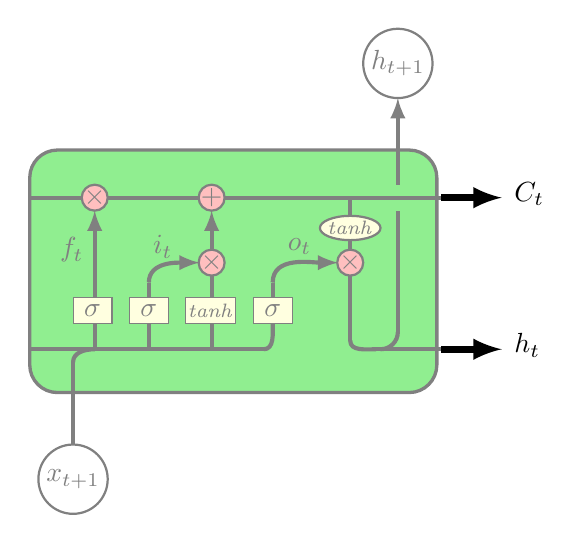
\begin{tikzpicture}[scale=1.1]

  % The grid
  % \draw[step=0.5, gray!40, very thin] (0,0) grid (8,4);

  % LSTM frame
  \def \yONE {0.5}
  \def \yTWO {3.3}
  \draw[rounded corners=10pt, very thick, gray,fill=LightGreen]  (1.5, 0.5) rectangle (6.2, 3.3);

  \def \sigmoidWidth  {0.45}
  \def \sigmoidInDist {0.2}
  \def \sigmoidHeight  {0.3}
  \def \yB  {1.3}
  \def \yD  {2.75}
  \def \shift {0.3}
  % First Sigmoid
  \draw[gray,fill=LightYellow] (2, \yB) rectangle (2+ \sigmoidWidth, \yB + \sigmoidHeight) node[pos=0.5] {$\sigma$};

  \def \r {.15cm}
  % The Upper times operator % first time from left
  \draw[thick, gray,fill=pink] (2.25, \yD) circle (\r) node {$\times$};

  % Second Sigmoid
  \def \xS {2.45 +\sigmoidInDist}
  \draw[gray,fill=LightYellow]  (\xS, \yB) rectangle (\xS +\sigmoidWidth, \yB + \sigmoidHeight) node[pos=0.5] {$\sigma$};

  % Square tanh
  \def \xSS {\xS +\sigmoidWidth + \sigmoidInDist}
  \draw[gray,fill=LightYellow]  (\xSS, \yB) 
  rectangle 
  (\xSS +\sigmoidWidth +0.13, \yB +\sigmoidHeight)
  node[pos=0.5] {\scriptsize \textit{tanh}};

  % Third Sigoid
  \def \xSSS {\xSS +\sigmoidWidth +0.13 +\sigmoidInDist}
  \draw[gray,fill=LightYellow]  (\xSSS, \yB) rectangle (\xSSS +\sigmoidWidth, \yB +\sigmoidHeight)
  node[pos=0.5] { $\sigma$};

  % Second times operator and add operator
  \def \xTimesB {3.6}
  \def \yC      {2}

  \draw[thick,gray,fill=pink] (\xTimesB, \yC) circle (\r) node {$\times$};
  %%%%% first line sectond operator +
  \draw[thick, gray,fill=pink] (\xTimesB, \yD) circle (\r) node {$+$};

  % Third times operator and its tanh
  \draw[thick,gray,fill=pink] (\xTimesB +1.3 +\shift, \yC) circle (\r) node {$\times$};
  \draw[thick,gray,fill=LightYellow] (\xTimesB +1.3 +\shift, \yC +.4)  
  ellipse (.35cm and .14cm) 
  node {\scriptsize \textit{tanh}};


  % LINES %%% Upper line from c_{t -1} till C_t
  %\draw[arrows=-latex, line width=2.5pt]  (0.85, \yD) -- (1.5, \yD) node[left, xshift=-.6cm, yshift=0.2cm] {$C_{t-1}$};
  \draw[line width=1.5pt,gray]  (1.5, \yD) -- (2.1, \yD);
  \draw[line width=1.5pt,gray]  (2.4, \yD) -- (3.46, \yD);
  \draw[line width=1.5pt,gray]  (3.75, \yD) -- (6.25 +0.2, \yD);

  \draw[arrows=-latex, line width=2.5pt]  (6.25, \yD) -- (6.75 +0.2, \yD)
  node[right, xshift=0.0cm, yshift=0.05cm] {$C_t$};

  %%%%first line from left from sigmoid ft till times input from C_{t-1}
  \draw[arrows=-latex, line width=1.5pt,gray]  (2.25, \yB +\sigmoidHeight) -- (2.25, 2.6)
  node[left, yshift=-0.5cm] {$f_t$};

  % Level B LINES
  \def \levelB {1}
  %\draw[arrows=-latex, line width=1.5pt,gray] (0.85, \levelB) -- (1.5, \levelB) node[left, xshift=-.6cm, yshift=0.2cm] {$h_{t-1}$};

  \draw[line width=1.5pt,gray] (1.5, \levelB) 
  --
  (4.2, \levelB);

  \def \xOfThirdSigmoid {\xSSS + \sigmoidWidth/2}
  %second line last angle connected to sigmoid 
  \draw[line width=1.5pt,gray] (4.2, \levelB) to[out=0,in=270] (\xOfThirdSigmoid, \yB);

  % Third Sigmoid up line
  % END (\xTimesB +1.3 - 0.19 , \yC)
  \draw[line width=1.5pt,gray] (\xOfThirdSigmoid, \yB + \sigmoidHeight) 
  --
  (\xOfThirdSigmoid, \yB + \sigmoidHeight + 0.17) ;

  \draw[arrows=-latex, line width=1.5pt,gray] (\xOfThirdSigmoid, \yB + \sigmoidHeight+0.17) 
  to[out=90, in=180] 
  (\xTimesB +1.3 -0.14 +\shift , \yC) 
  node [left, yshift=0.2cm, xshift=-0.2cm] {$o_t$};

  % tanh line
  \draw [line width=1.5pt,gray] (\xTimesB, \levelB)
  --
  (\xTimesB, \yB);

  \draw [line width=1.5pt,gray] (\xTimesB, \yB + \sigmoidHeight)
  --
  (\xTimesB, \yB + \sigmoidHeight +0.24);

  \draw [arrows=-latex, line width=1.5pt,gray] (\xTimesB, 2.15)
  --
  (\xTimesB, 2.6);

  \draw[line width=1.5pt,gray] (2.25, \levelB)
  --
  (2.25, \yB);
  
  \draw[line width=1.5pt,gray] (\xS +\sigmoidWidth/2, \levelB)
  --
  (\xS +\sigmoidWidth/2, \yB);

  \draw[line width=1.5pt,gray] (\xS +\sigmoidWidth/2, \yB +\sigmoidHeight)
  -- 
  (\xS +\sigmoidWidth/2, \yB +\sigmoidHeight + 0.17);

  \draw[arrows=-latex, line width=1.5pt,gray] (\xS +\sigmoidWidth/2, \yB + \sigmoidHeight+0.17) 
  to[out=90, in=180] 
  (\xTimesB-0.14, \yC)
  node [left, yshift=0.2cm, xshift=-0.2cm] {$i_t$};

  \def \bigR {0.25cm}
  \def \bigRTWO {0.4cm}
  \def \C    {1}
  \def \xBigCicleONE {2}
  \def \xBigCicleTWO {5.5 + 0.25}
  \draw[thick,gray] (\xBigCicleONE, \yONE - \C) circle (\bigRTWO) node {$x_{t+1}$};
  \draw[thick,gray] (\xBigCicleTWO, \yTWO + \C) circle (\bigRTWO) node {$h_{t+1}$};

  % LINE Circle ONE
  \draw[line width=1.5pt,gray] (\xBigCicleONE, \yONE -\C +0.4) 
  --
  (\xBigCicleONE, \yONE -\C +0.25 + 1.1);

  \draw[line width=1.5pt,gray] (\xBigCicleONE, \yONE -\C +0.25 + 1.1)
  to[out=90, in=180]
  (2.25, 1);

  % LINE third \times
  \draw[line width=1.5pt,gray] (\xTimesB +1.3 +\shift, 1.1)
  --
  (\xTimesB +1.3 +\shift, \yC - 0.15);

  \draw[line width=1.5pt,gray] (5.5, 1) 
  --
  (6.25 +0.2, 1);
  
  \draw[arrows=-latex,line width=2.5pt] (6.25, 1) 
  --
  (6.75 +0.2, 1)
  node[right, xshift=0.0cm, yshift=0.05cm,] {$h_t$};

%%% second line last angle connect the input with h_t output
  \draw[line width=1.5pt,gray] (\xTimesB +1.3 +\shift, 1.1)
  to[out=270, in=180]
  (5.5, 1);


  \draw[line width=1.5pt,gray] (\xTimesB +1.3 +\shift, 2.14)
  --
  (\xTimesB +1.3 +\shift, 2.26);


  \draw[line width=1.5pt,gray] (\xTimesB +1.3 +\shift, \yD)
  --
  (\xTimesB +1.3 +\shift, 2.54);


  \draw[line width=1.5pt,gray] (\xBigCicleTWO, \levelB +0.2)
  --
  (\xBigCicleTWO, 2.6);

%%%%% first horizontal line from the right angle connected to output ht
  \draw[line width=1.5pt,gray] (\xBigCicleTWO - 0.2, \levelB)
  to[out=0, in=270]
  (\xBigCicleTWO, \levelB +0.2);


  \draw[arrows=-latex, line width=1.5pt,gray]
  (\xBigCicleTWO, \yD +0.15)
  --
  (\xBigCicleTWO, 4-.1);

\end{tikzpicture}

\endminipage

\caption{The repeating module in an LSTM contains four interacting layers.\cite{colah}}
\label{fig:LSTM-cell-chaining}
\end{figure}

